\documentclass[12pt]{article} % Sets the font size to 12pt and defines the document as an article

\usepackage[
backend=biber, 
citestyle=ieee,
sorting=nyt,    
doi=false,
url=false,
isbn=false,
giveninits=true,
maxbibnames=9999,
hyperref]{biblatex}

\addbibresource{CS250.bib} 

% Packages for mathematical fonts and symbols
\usepackage{amsfonts, amssymb, amsmath}
\usepackage{booktabs}
\usepackage{float}
\usepackage{ulem}
\usepackage{tabularx}
\usepackage[ruled,vlined]{algorithm2e}
\usepackage{graphicx}


% Uncomment the following lines if you want to enable double spacing
%\usepackage{setspace}
%\doublespacing

% Margin settings
\usepackage[margin=1in]{geometry} % Simplifies margin settings using the geometry package

% Header and footer customization
\usepackage{fancyhdr}

\pagestyle{fancy}
\fancyhf{} % Clears default header and footer
\fancyhead[L]{CS250/homework5/JuntangWang} 
\fancyhead[C]{\today} 
\fancyhead[R]{\thepage} 

% Custom commands
\newcommand{\eqn}{\begin{array}{rcl}} % Begin an aligned equation environment
\newcommand{\eqnend}{\end{array}}    % End the aligned equation environment
\newcommand{\qed}{\hfill $\square$} % End of proof symbol

% Title Information
\title{CS521 Homework5} % Replace with your actual title
\author{Juntang Wang}        % Replace with your actual name
\date{\today}             % Automatically uses the current date

\begin{document}

\section{Q1}
\subsection{(a)}
\textbf{Solution:}

\textbf{Step 1: Convert the Hex String to Binary}

First, convert each hex digit to its 4-bit binary equivalent:

\[
\begin{array}{ccccccccc}
\text{Hex:} & 2 & 0 & A & 3 & 0 & 0 & 1 & 2 \\
\text{Bin:} & 0010 & 0000 & 1010 & 0011 & 0000 & 0000 & 0001 & 0010 \\
\end{array}
\]

\textbf{Step 2: Identify the Opcode}

Opcode (bits 31-26): \(001000\). Which corresponds to the \texttt{ADDI} instruction in MIPS.  \cite{MIPS32}

\textbf{Step 3: Break Down the Binary Instruction}

MIPS instructions come in: R-type, I-type, and J-type. Based on the opcode, we can determine the format. The instruction format for I-type (which includes \texttt{ADDI}) is:

\begin{itemize}
    \item \textbf{Opcode (bits 31-26)}: \(001000\) (binary) \(= 8\) (decimal)
    \item \textbf{rs (bits 25-21)}: \(00101\) (binary) \(= \$5\) (register 5)
    \item \textbf{rt (bits 20-16)}: \(00011\) (binary) \(= \$3\) (register 3)
    \item \textbf{Immediate (bits 15-0)}: \(0000000000010010\) (binary) \(= 18\) (decimal)
\end{itemize}



\textbf{Step 4: Assemble the Instruction}

Now, we can construct the instruction:

\[
\boxed{
\texttt{addi \$3, \$5, 18}
}
\quad \text{or} \quad
\boxed{
\texttt{addi \$v1, \$a1, 18}
}
\]


\subsection{(c)}
\textbf{Solution:}

\noindent
Extract all the true output cases and take the sum:
\[
!A !B !C +
!A  B !C +
 A !B !C +
 A  B  C
\]

\noindent
Combining first and third terms
\(
(!A + A) !B !C = !B !C,
\)
we have:
\[
!B !C +
!A  B !C +
 A  B  C
\]

\noindent
Since $!A !B !C$ already covered in $!B !C$, s.t. $!A  B !C + !A !B !C = !A !C$

\noindent
combining first and second terms
\(
!B !C +
!A  B !C
= !B !C + !A !C
= !C(!A + !B)
\)
we have:
\[
\boxed{
!C(!A + !B) +
 A  B  C
}
\]

% ----------------------------------------------------------------
% Drafted by Juntang Wang 2024-10-21
% ----------------------------------------------------------------  


\section{Q3}
\subsection{(a)}
\textbf{Solution:}

\begin{figure}[h!]
    \centering
    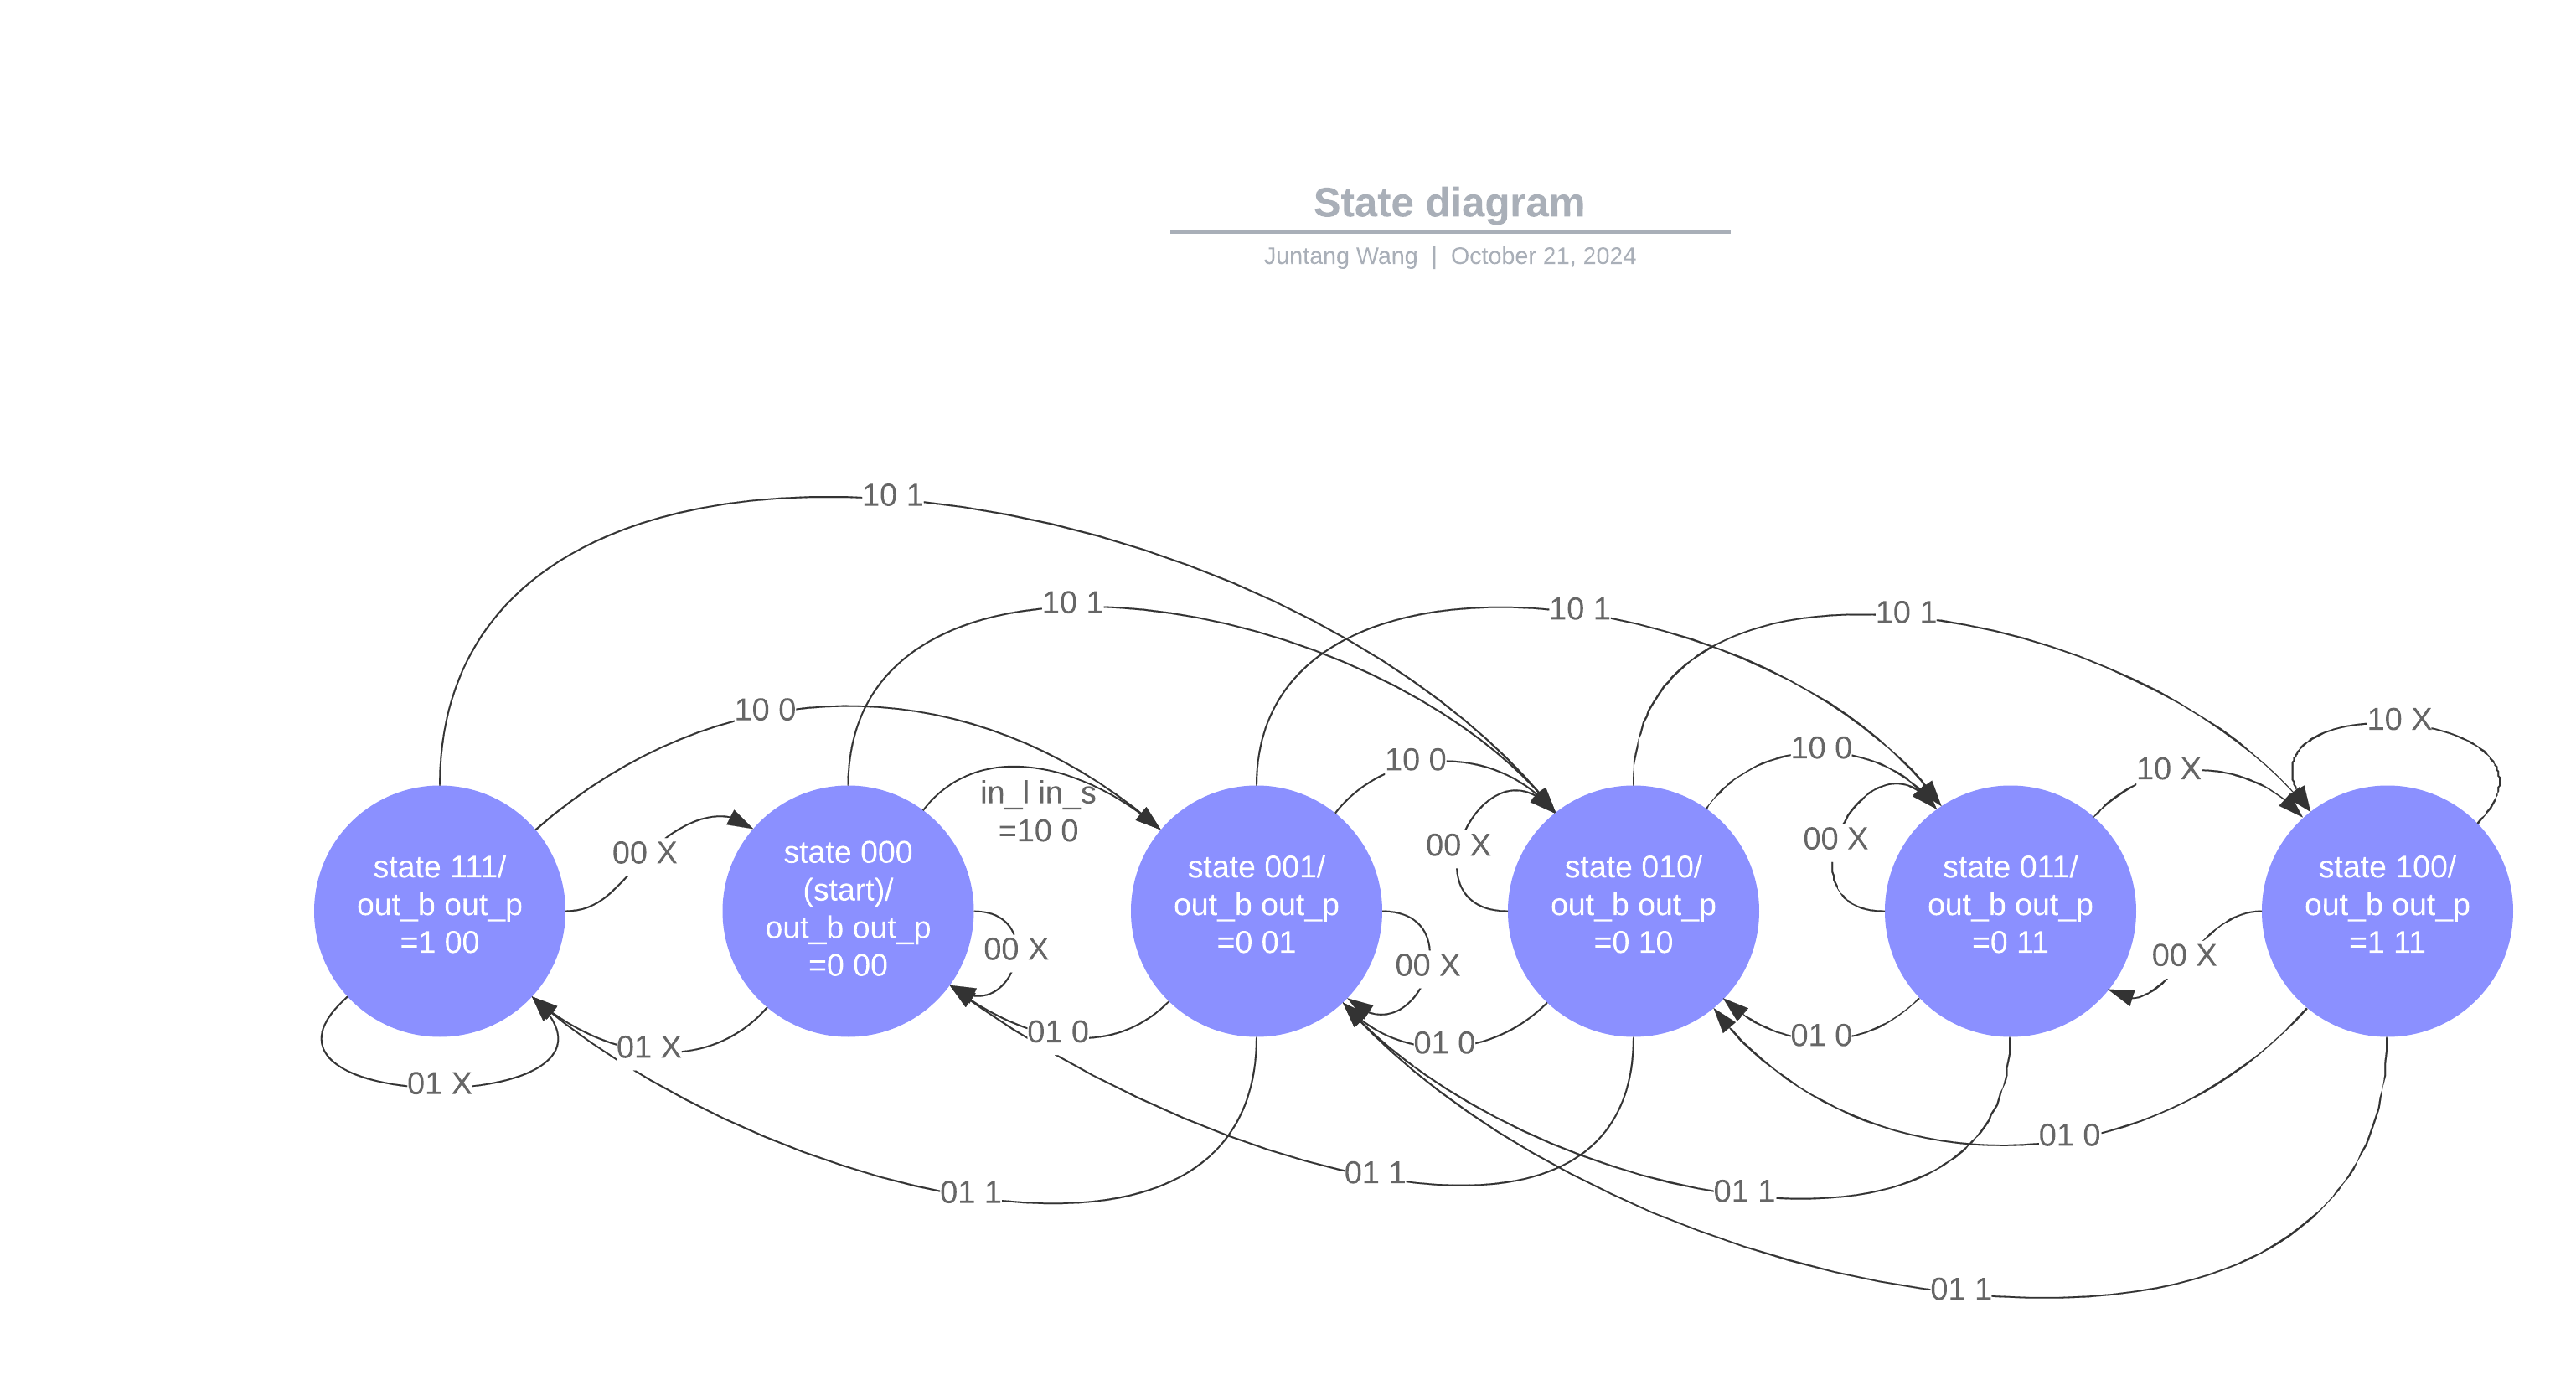
\includegraphics[width=0.8\textwidth]{figures/State diagram.png}
    \caption{State diagram for the FSM}
    \label{fig:state-diagram}
\end{figure}

Figure \ref{fig:state-diagram} shows the state diagram for the finite state machine (FSM). This diagram illustrates the states and transitions of the FSM based on the given specifications.

\begin{itemize}
    \item The FSM has six states: 100, 000, 001, 010, 011 and 111.
    \item Transitions between states occur based on the input\_leftright (input\_l) and input\_speed (input\_s).
    \item The output\_position (output\_p) and output\_blocked (output\_b) is determined by the current state.
\end{itemize}

The state diagram was created using Lucid Chart \cite{lucidchart}.

% ----------------------------------------------------------------
% Drafted by Juntang Wang 2024-10-21
% ----------------------------------------------------------------  

\subsection{(b)}
\textbf{Solution:}

\begin{table}[H]
    \centering
    \begin{tabular}{|c|c|c|c|c|c|c|c|c|c|c|c|}
        \hline
        Q0& Q1& Q2& out\_blocked & out\_position1&out\_position0& in\_leftright1 &in\_leftright0& in\_speed& D0& D1&D2\\
        \hline
        0 & 0 & 0 & 0  & 0  &0& 0&0& X& 0& 0&0\\ \hline 
 0 & 0 & 0 & 0  & 0  &0& 0& 1& X& 1& 1&1\\ \hline 
 0 & 0 & 0 & 0  & 0  &0& 1& 0& 0& 0& 0&1\\ \hline 
 0 & 0 & 0 & 0  & 0  &0& 1& 0& 1& 0& 1&0\\ \hline 
        0 & 0 & 1 & 0  & 0  &1& 0&0& X& 0& 0&1\\ \hline 
 0 & 0 & 1 &  0  & 0  &1& 0& 1& 0& 0& 0&0\\ \hline 
 0 & 0 & 1 &  0  & 0  &1& 0& 1& 1& 1& 1&1\\ \hline 
 0 & 0 & 1 &  0  & 0  &1& 1& 0& 0& 0& 1&0\\ \hline 
 0 & 0 & 1 &  0  & 0  &1& 1& 0& 1& 0& 1&1\\ \hline 
        0 & 1 & 0 & 0  & 1  &0& 0&0& X& 0& 1&0\\ \hline 
 0 & 1 & 0 & 0  & 1  & 0& 0& 1& 0& 0& 0&1\\ \hline 
 0 & 1 & 0 & 0  & 1  & 0& 0& 1& 1& 0& 0&0\\ \hline 
 0 & 1 & 0 & 0  & 1  & 0& 1& 0& 0& 0& 1&1\\ \hline 
 0 & 1 & 0 & 0  & 1  & 0& 1& 0& 1& 1& 0&0\\ \hline 
        0 & 1 & 1 & 0 & 1&1& 0&0& X& 0& 1&1\\ \hline 
 0 & 1 & 1 & 0 & 1& 1& 0& 1& 0& 0& 1&0\\ \hline 
 0 & 1 & 1 & 0 & 1& 1& 0& 1& 1& 0& 0&1\\ \hline 
 0 & 1 & 1 & 0 & 1& 1& 1& 0& X& 1& 0&0\\ \hline 
        1 & 0 & 0 & 1 & 1&1& 0&0& X& 0& 1&1\\ \hline 
 1 & 0 & 0 & 1 & 1& 1& 0& 1& 0& 0& 1&0\\ \hline 
 1 & 0 & 0 & 1 & 1& 1& 0& 1& 1& 0& 0&1\\ \hline 
 1 & 0 & 0 & 1 & 1& 1& 1& 0& X& 1& 0&0\\ \hline 
        1& 0& 1&  \multicolumn{9}{|c|}{No Such State}\\ \hline 
        1& 1& 0&  \multicolumn{9}{|c|}{No Such State}\\ \hline 
        1 & 1 & 1 & 1 & 0&0& 0&0& X& 0& 0&0\\ \hline
 1 & 1 & 1 & 1 & 0& 0& 0& 1& X& 1& 1&1\\ \hline 
 1 & 1 & 1 & 1 & 0& 0& 1& 0& 0& 0& 0&1\\ \hline 
 1 & 1 & 1 & 1 & 0& 0& 1& 0& 1& 0& 1&0\\ \hline
    \end{tabular}
    \caption{}
    \label{tab:truth_table}
\end{table}

% ----------------------------------------------------------------
% Drafted by Juntang Wang 2024-10-21
% ----------------------------------------------------------------  


\printbibliography

\end{document}

% ----------------------------------------------------------------
% Drafted by Juntang Wang 2024-10-21
% ----------------------------------------------------------------
